\documentclass[11pt, oneside]{article}   	% use "amsart" instead of "article" for AMSLaTeX format
\usepackage{geometry}                		% See geometry.pdf to learn the layout options. There are lots.
\geometry{letterpaper}                   		% ... or a4paper or a5paper or ... 
%\geometry{landscape}                		% Activate for rotated page geometry
%\usepackage[parfill]{parskip}    		% Activate to begin paragraphs with an empty line rather than an indent
\usepackage{graphicx}				% Use pdf, png, jpg, or eps§ with pdflatex; use eps in DVI mode
								% TeX will automatically convert eps --> pdf in pdflatex		
\usepackage{amssymb}

%SetFonts

%SetFonts


\title{SitePassword Modulo Bias}
\author{Alan H. Karp}
%\date{}							% Activate to display a given date or no date

\begin{document}
\maketitle
\abstract

SitePassword hashes  a super password, a per site nickname, and a per site userid to produce a site password.  The bytes produced by the hash need to be converted to a string of characters selected from the alphabet supported by the web site associated with that user account.  In some situations, {\em modulo bias} reduces the entropy of the site password.  This note shows that the effect is modest for the range of values SitePassword supports.

\section{Introduction}

The original SitePassword algorithm used each byte of the hash produced by PBKDF2\footnote{Password Based Key Derivation Function} to compute the $i$-th character of the site password using $c_i = A[b_i  \bmod  |A|)]$, where $A$ is an array of characters representing the alphabet, $b_i$ is the byte value, and $|A|$ is the size of the alphabet.  If the size of the alphabet evenly divides $2^8 = 256$, every character in the alphabet has the same probability of being selected.  If it doesn't, then some characters are more likely to be selected.  This {\em modulo bias} reduces the entropy of the resulting string.  
 

This document shows that modulo bias has only a modest effect on the guessability of the site password it generates.

\section{Recommended Approaches}

The recommended approach to eliminating modulo bias is {\em rejection sampling}.  Simply ignore any byte value index outside the range of the alphabet.  In other words, don't use any $b_i > |A|$.  Theoretically, this approach could require an unbounded number of bytes, but the number of bytes needed is modest in practice.  

Usability considerations require that SitePassword always succeed in computing a password, which means it must be conservative in how many bytes it computes with rejection sampling.  While it's possible to estimate how many extra bytes are needed to achieve a given probability of success, there are no guarantees.  

A second problem with rejection sampling is that it makes offline guessing of the super password easier.  The runtime of PBKDF2 depends on the number of iterations and the key size.  In order to have a high enough probability of having enough bytes left after rejection, SitePassword must compute a very large number of bytes.  An adversary who is willing to give up guessing the super password for a small fraction of site passwords can compute fewer bytes.

Consider an example with SitePassword's default parameters.  A failure rate of one in a million requires computing 50 bytes/character in the password.  An adversary who is willing to succeed only 99\% of the time would need to compute 16 characters/byte, gaining a 3x computational advantage.

One workaround would be for SitePassword to first compute a key with a modest number of bytes, say 2 times the size of the site password.  If more bytes are needed, SitePassword could redo the calculation with the first set of bytes as input.  Unfortunately, the fixed overhead of each run makes it hard to meet the latency requirement.

The recommended approach to mitigating modulo bias is to use a larger range of random numbers, say two bytes instead of one.  There is still bias, but the effect on guessability is substantially smaller.

\section{Quantifying Modulo Bias}

There will be no need to use extra bytes to construct the site password if modulo bias doesn't weaken the site password very much.  One way to quantify that weakening is by looking at the entropy of the site password both with and without modulo bias.  Without bias, the entropy of an $L$-character site password is 

\begin{equation}
E_0 = L \log_2 |A|
\end{equation}

The easiest way to understand modulo bias is to keep repeating the alphabet until the result is has more elements than the largest possible random value $R$ and truncate to size $R$.  If $|A|$ doesn't evenly divide $R$, some characters will appear one more time than others.  The number of times a character appears is either
\begin{equation}
n_1 = \lfloor R/|A| \rfloor ~~\textrm{or}~~ n_2 = \lceil R/|A| \rceil,
\end{equation}
so that $n_1 = n_2$ if $|A|$ divides $R$ or $n_2 = n_1 + 1$ otherwise.  The probabilities that one of those characters is chosen is, 
\begin{equation}
p_1 = n_1/R ~~\textrm{or}~~ p_2 = n_2/R.
\end{equation}

The entropy of selecting a single character from each subset is then
\begin{equation}
E_1 = -(|A| - R \bmod |A]) p_1 \log_2 p_1 ~~~\textrm{or}~~ E_2 = - (R \bmod |A|) p_2 \log_2 p_2.
\end{equation}

Here ($R \bmod|A|$) is the number of characters that appear an extra time.  Note that if $|A|$ divides $R$, $E_2 = 0$ and $E_1 = E_0$.  The entropy of an $L$-character site password with modulo bias is $E_b = L(E_1 + E_2)$.  

\begin{figure}
    \centering
    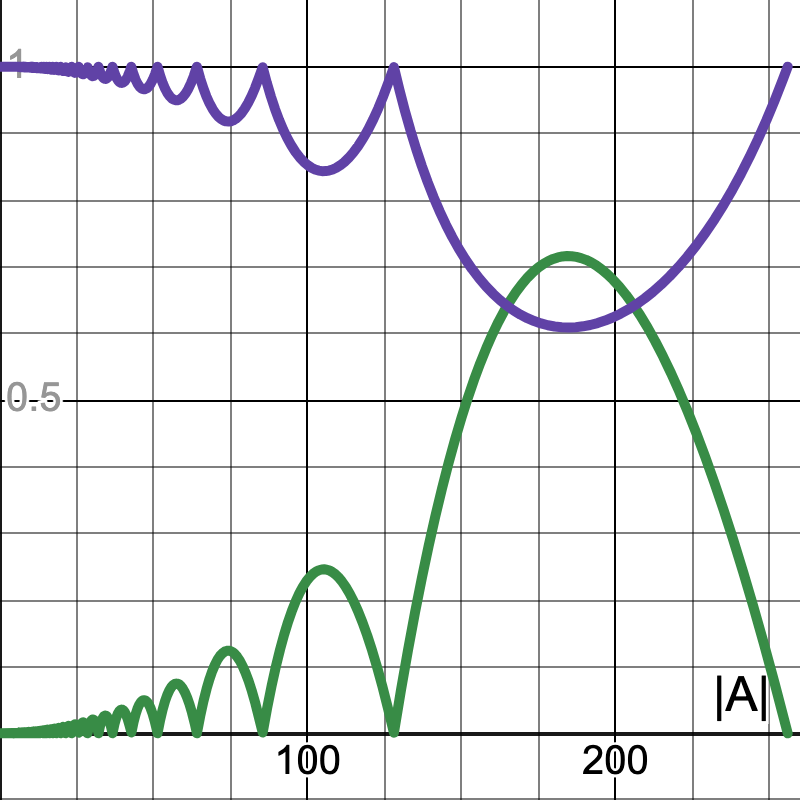
\includegraphics[width=0.5\textwidth]{moduloBias.png} 
    \caption{Modulo bias for SitePassword for an $L$-character site password.  The green line is the entropy loss; the purple line the reduction in the number of guesses.  Only values of $10 \leq |A| \leq 96$ are relevant to SitePassword.}
    \label{fig}
\end{figure}

We can now plug in some numbers.  SitePassword uses $R = 256$ and allows alphabets in the range $10 \leq |A| \leq 96$.  With the default values of $|A| = 62$ and $L = 12$, $E_0 - E_b = .05$ which requires 96\% of the $2^{71}$ guesses needed if there was no modulo bias.  The worst case in the allowed range is at $|A| = 96$ where $E_0 - E_b = 0.28$, which translates into 82\% as many guesses.  The greater loss in guesses is offset by the larger alphabet size, leaving the entropy with modulo bias greater than 78 bits.  Figure~\ref{fig} shows the entropy loss, $E_0 - E_b$, in green and the ratio of the number of guesses needed, $2^{-(E_0-E_b)}$, in purple for $R = 256$ and $L = 12$.

\section{Conclusions}

There are cases where a small modulo bias can be a serious problem, such as in choosing a nonce for a stream cypher.  That is not the case for SitePassword.  Even the most extreme modulo bias reduces the entropy of the site password by less than one bit.  Even so, the SitePassword algorithm was changed to use 2 bytes per character, which makes the modulo bias considerably smaller.

\end{document}  